%%%%%%%% ICML 2026 EXAMPLE LATEX SUBMISSION FILE %%%%%%%%%%%%%%%%%

\documentclass{article}

% Recommended, but optional, packages for figures and better typesetting:
\usepackage{microtype}
\usepackage{graphicx}
\usepackage{subcaption}
\usepackage{booktabs} % for professional tables

% hyperref makes hyperlinks in the resulting PDF.
% If your build breaks (sometimes temporarily if a hyperlink spans a page)
% please comment out the following usepackage line and replace
% \usepackage{icml2026} with \usepackage[nohyperref]{icml2026} above.
\usepackage{hyperref}


% Attempt to make hyperref and algorithmic work together better:
\newcommand{\theHalgorithm}{\arabic{algorithm}}

% Use the following line for the initial blind version submitted for review:
\usepackage{icml2026}

% For preprint, use
% \usepackage[preprint]{icml2026}

% If accepted, instead use the following line for the camera-ready submission:
% \usepackage[accepted]{icml2026}

\usepackage{amsmath}
\usepackage{amssymb}
\usepackage{mathtools}
\usepackage{amsthm}


% if you use cleveref..
\usepackage[capitalize,noabbrev]{cleveref}

% ---- Packages ----
\usepackage{microtype}
\usepackage{graphicx}
\usepackage{subcaption}
\usepackage{booktabs}
\usepackage{multirow}
\usepackage{amsmath, amssymb, amsfonts}
\usepackage{mathtools}
\usepackage{bm}
\usepackage{algorithm}
\usepackage{algorithmic}
\usepackage{hyperref}
\usepackage{cleveref}
% \usepackage{enumitem}
\usepackage[inline, shortlabels]{enumitem}
\usepackage{xcolor}
\usepackage{amsthm}

% ---- Optional: TikZ for figures ----
\usepackage{tikz}
\usetikzlibrary{positioning, arrows.meta, calc}

% ---- Handy commands (edit later) ----
\newcommand{\wm}{\textsc{WM}}
\newcommand{\mawm}{\textsc{MAWM}}
\newcommand{\nsm}{\textsc{NS-MAWM}}
\newcommand{\DecPOMDP}{\textsc{Dec-POMDP}}
\newcommand{\RVR}{\textsc{RVR}}
\newcommand{\KL}{\mathrm{KL}}

% --- Tickz
\usepackage{physics}
\usepackage{tikz}
\usetikzlibrary{arrows.meta,positioning,fit,calc}
\usepackage{amsmath}
\usepackage{mathdots}
% \usepackage{yhmath}
\usepackage{cancel}
\usepackage{color}
\usepackage{siunitx}
\usepackage{array}
\usepackage{multirow}
% \usepackage{amssymb}
\usepackage{gensymb}
\usepackage{tabularx}
\usepackage{extarrows}
\usepackage{booktabs}
\usetikzlibrary{fadings}
\usetikzlibrary{patterns}
\usetikzlibrary{shadows.blur}
\usetikzlibrary{shapes}

% ---- Math shortcuts ----
\newcommand{\E}{\mathbb{E}}
\newcommand{\R}{\mathbb{R}}
\newcommand{\I}{\mathbb{I}}

\usepackage{amssymb}
\usepackage{pifont}

\newcommand{\cmark}{\ding{51}}%
\newcommand{\xmark}{\ding{55}}%

\usepackage[english]{babel}
\addto\extrasenglish{  
    \def\figureautorefname{Figure}
    \def\tableautorefname{Table}
    \def\algorithmautorefname{Algorithm}
    \def\sectionautorefname{Section}
    \def\subsectionautorefname{Subsection}
    \def\proofoutlineautorefname{Proof Outline}
}

%%%%%%%%%%%%%%%%%%%%%%%%%%%%%%%%
% THEOREMS
%%%%%%%%%%%%%%%%%%%%%%%%%%%%%%%%
\theoremstyle{plain}
\newtheorem{theorem}{Theorem}[section]
\newtheorem{proposition}[theorem]{Proposition}
\newtheorem{lemma}[theorem]{Lemma}
\newtheorem{corollary}[theorem]{Corollary}
\theoremstyle{definition}
\newtheorem{definition}[theorem]{Definition}
\newtheorem{assumption}[theorem]{Assumption}
\theoremstyle{remark}
\newtheorem{remark}[theorem]{Remark}

% Todonotes is useful during development; simply uncomment the next line
%    and comment out the line below the next line to turn off comments
%\usepackage[disable,textsize=tiny]{todonotes}
\usepackage[textsize=tiny]{todonotes}

% The \icmltitle you define below is probably too long as a header.
% Therefore, a short form for the running title is supplied here:
\icmltitlerunning{Neuro-Symbolic Multi-Agent World Models}

\begin{document}

\twocolumn[
  \icmltitle{Invariant-Aware Neuro-Symbolic Multi-Agent World Models\\
    for Model-Based Multi-Agent Reinforcement Learning}

  % It is OKAY to include author information, even for blind submissions: the
  % style file will automatically remove it for you unless you've provided
  % the [accepted] option to the icml2026 package.

  % List of affiliations: The first argument should be a (short) identifier you
  % will use later to specify author affiliations Academic affiliations
  % should list Department, University, City, Region, Country Industry
  % affiliations should list Company, City, Region, Country

  % You can specify symbols, otherwise they are numbered in order. Ideally, you
  % should not use this facility. Affiliations will be numbered in order of
  % appearance and this is the preferred way.
  \icmlsetsymbol{equal}{*}

  \begin{icmlauthorlist}
    \icmlauthor{Julien Soulé}{equal,yyy}
    \icmlauthor{Georgios Bakirtzis}{equal,yyy,comp}
    \icmlauthor{Jean-Paul Jamont}{comp}
    \icmlauthor{Firstname4 Lastname4}{sch}
    \icmlauthor{Firstname5 Lastname5}{yyy}
    \icmlauthor{Firstname6 Lastname6}{sch,yyy,comp}
    \icmlauthor{Firstname7 Lastname7}{comp}
    %\icmlauthor{}{sch}
    \icmlauthor{Firstname8 Lastname8}{sch}
    \icmlauthor{Firstname8 Lastname8}{yyy,comp}
    %\icmlauthor{}{sch}
    %\icmlauthor{}{sch}
  \end{icmlauthorlist}

  \icmlaffiliation{yyy}{Department of XXX, University of YYY, Location, Country}
  \icmlaffiliation{comp}{Company Name, Location, Country}
  \icmlaffiliation{sch}{School of ZZZ, Institute of WWW, Location, Country}

  \icmlcorrespondingauthor{Julien Soulé}{julien.soule@hotmail.fr}
  \icmlcorrespondingauthor{Firstname2 Lastname2}{first2.last2@www.uk}

  % You may provide any keywords that you find helpful for describing your
  % paper; these are used to populate the "keywords" metadata in the PDF but
  % will not be shown in the document
  \icmlkeywords{Machine Learning, ICML}

  \vskip 0.3in
]

% this must go after the closing bracket ] following \twocolumn[ ...

% This command actually creates the footnote in the first column listing the
% affiliations and the copyright notice. The command takes one argument, which
% is text to display at the start of the footnote. The \icmlEqualContribution
% command is standard text for equal contribution. Remove it (just {}) if you
% do not need this facility.

% Use ONE of the following lines. DO NOT remove the command.
% If you have no special notice, KEEP empty braces:
\printAffiliationsAndNotice{}  % no special notice (required even if empty)
% Or, if applicable, use the standard equal contribution text:
% \printAffiliationsAndNotice{\icmlEqualContribution}

% ============================
% Abstract
% ============================
\begin{abstract}
  % TODO: 6--10 lines.
  % Problem: MA world models under partial observability suffer from semantic drift / inconsistency.
  % Idea: inject neuro-symbolic invariants / equivariances as soft constraints (optionally gated).
  % Method: NS-MAWM training with WM loss + rule consistency regularizer.
  % Results: better long-horizon prediction, lower rule violation, improved downstream planning/RL and generalization.
  % Contributions: framework + metrics + experiments.

  Model-based reinforcement learning enables planning through learned world models, but extending these approaches to multi-agent settings is difficult due to partial observability and error accumulation in joint observation dynamics. Purely neural multi-agent world models often produce semantically inconsistent predictions, violating spatial coherence, object persistence, and interaction constraints.
  We introduce \textbf{Neuro-Symbolic Multi-Agent World Models (NS-MAWM)}, which incorporate symbolic invariants and action-conditioned equivariances as differentiable consistency constraints during world model training. These constraints act as structured inductive biases that reduce long-horizon semantic drift while preserving uncertainty through soft satisfaction. An optional gating mechanism learns when rules should be applied, avoiding over-constraining in stochastic environments.
  Experiments on grid-based multi-agent environments and a standard benchmark show that NS-MAWM improves long-horizon prediction consistency, downstream planning performance, and generalization compared to neural baselines.

\end{abstract}

% ============================
% 1. Introduction
% ============================
\section{Introduction}
\label{sec:intro}
% TODO:
% - Context: model-based RL + world models; multi-agent adds partial observability + non-stationarity + joint observation dynamics.
% - Failure mode: semantic inconsistency, long-horizon drift, hallucinated objects, broken geometry.
% - Key idea: neuro-symbolic invariants/equivariances as structured inductive biases / constraints.
% - Summary of contributions (bullets).
% - Outline.

Model-based reinforcement learning (MBRL) has emerged as a powerful paradigm for data-efficient decision making by learning predictive \emph{world models} that support planning, imagination, and counterfactual reasoning \cite{ha2018worldmodels,hafner2019learning,hafner2020dreamer}. By rolling out learned dynamics in latent space, agents can reason over future trajectories without interacting with the environment, enabling substantial gains in sample efficiency and control performance \cite{Racaniere2017imagination}. Extending these ideas to multi-agent reinforcement learning (MARL) is particularly appealing, as many real-world systems involve multiple interacting agents operating under partial observability and decentralized control \cite{oliehoek2016concise,nguyen2020deep,zhang2021}. However, despite growing interest in model-based MARL \cite{Xu2022mingling,Venugopal2024MABL}, learning reliable \emph{multi-agent world models} remains a largely open problem.

In multi-agent settings, world models must predict not only environmental dynamics but also the joint effects of multiple agents’ actions on local, partial observations. Purely neural world models often produce predictions that are statistically plausible yet semantically inconsistent, especially over long-horizon rollouts \cite{talvitie2014modelbias,venkatraman2015improving}. Objects may appear or disappear without cause, spatial relations may be violated, and interaction constraints may be broken, resulting in compounding errors that undermine planning and imagination \cite{zhang2021worldmodelgraph}. Addressing \emph{semantic correctness}, rather than only predictive accuracy, is therefore essential for multi-agent world models to function as reliable internal simulators.

We argue that the difficulty of learning reliable multi-agent world models stems from several distinct but interrelated gaps in existing approaches:

\begin{itemize}
  \item \textbf{(G1) Absence of explicit semantic invariants.}
        Most world models are trained end-to-end from data without explicitly encoding invariants such as object permanence, spatial coherence, or exclusivity. These properties must be discovered implicitly from observations, often unreliably, especially under partial observability \cite{kipf2020contrastivelearningstructuredworld,zhang2021worldmodelgraph}.

  \item \textbf{(G2) Lack of action-conditioned equivariance constraints.}
        In many environments, agents’ actions induce structured transformations of observations, such as translations or rotations. While equivariant representations have proven effective in reinforcement learning \cite{mondal2022eqr,park2022learning}, they are rarely enforced within multi-agent world models and are typically not conditioned on agents’ actions.

  \item \textbf{(G3) Over-constraining versus uncertainty under partial observability.}
        Introducing structure through hard constraints can be brittle in stochastic or partially observable environments. Existing approaches lack mechanisms to apply constraints selectively, balancing prior knowledge with uncertainty \cite{oliehoek2016concise,Wong2023}.

  \item \textbf{(G4) Missing evaluation of semantic consistency.}
        Standard evaluation metrics for world models focus on reconstruction or prediction error, which fail to capture semantic violations critical for long-horizon reasoning. As a result, models with similar predictive accuracy may differ substantially in their suitability for planning \cite{Duan_2025_ICCV}.
\end{itemize}

Although prior work addresses parts of this global problem (through model-based MARL \cite{Xu2022mingling,Venugopal2024MABL}, structured or object-centric representations \cite{kipf2020contrastivelearningstructuredworld}, equivariant architectures \cite{mondal2022eqr,park2022learning}, or neuro-symbolic learning \cite{manhaeve2018deepproblog,balloch2023neurosymbolicworldmodelsadapting}) these lines of research largely evolve in isolation. Consequently, none of them jointly ensure semantic invariants, uncertainty-aware constraint application, and principled evaluation in multi-agent world models.

In this work, we propose \emph{Neuro-Symbolic Multi-Agent World Models (NS-MAWM)}, a framework designed to explicitly fill these gaps. Our key idea is to integrate symbolic invariants and action-conditioned equivariances into multi-agent world model training as \emph{soft, differentiable consistency constraints}. These constraints act as structured inductive biases that restrict the space of plausible dynamics while preserving uncertainty. To avoid over-constraining the model under partial observability, we introduce a learned gating mechanism that determines when symbolic rules should be applied.

Finally, we introduce a novel evaluation metric, the \emph{Rule Violation Rate}, which measures semantic consistency over long-horizon rollouts by quantifying violations of predefined invariants. Through extensive experiments on grid-based multi-agent environments and a standard multi-agent benchmark, we show that enforcing neuro-symbolic consistency significantly reduces semantic drift, improves long-horizon prediction fidelity, and leads to better downstream planning performance and generalization compared to purely neural baselines.

The remainder of the paper is organized as follows.
\autoref{sec:related} reviews related work on world models, model-based multi-agent reinforcement learning, equivariant representations, and neuro-symbolic approaches, and positions our contributions with respect to the identified gaps.
\autoref{sec:background} introduces the decentralized partially observable multi-agent reinforcement learning setting and formalizes multi-agent world models.
\autoref{sec:method} presents the proposed Neuro-Symbolic Multi-Agent World Model framework, including the rule language, differentiable consistency loss, and optional gating mechanism.
\autoref{sec:analysis} provides an analysis of how consistency constraints mitigate long-horizon semantic drift in learned world models.
\autoref{sec:eval} describes the experimental setup, evaluation metrics, baselines, and empirical results.
Finally, \autoref{sec:conclusion} concludes the paper and discusses limitations and future research directions.

% ============================
% 3. Related Work
% ============================

\section{Related work}
\label{sec:related}

We review prior work through the lens of the four gaps identified in the Introduction: semantic invariants (G1), action-conditioned equivariance (G2), uncertainty-aware constraint application (G3), and semantic evaluation of world models (G4).

\subsection{World Models and Model-Based Reinforcement Learning}

World models were introduced as latent generative models that enable agents to predict future observations and rewards for planning and imagination \cite{ha2018worldmodels}. Subsequent work demonstrated that learning compact latent dynamics can significantly improve sample efficiency and control performance \cite{hafner2019learning,hafner2020dreamer,Racaniere2017imagination}. However, these approaches focus primarily on single-agent settings and evaluate world models based on reconstruction accuracy or task performance, without explicitly addressing semantic consistency over long horizons.

Several works have investigated long-horizon prediction errors and compounding model bias in learned dynamics \cite{talvitie2014modelbias,venkatraman2015improving}. Graph-based and landmark-based world models attempt to mitigate such issues by introducing structured latent representations \cite{zhang2021worldmodelgraph}, yet they still rely on purely neural training objectives and do not enforce explicit semantic invariants.

\subsection{Model-Based Multi-Agent Reinforcement Learning}

Extending world models to multi-agent reinforcement learning introduces additional challenges due to decentralized control, partial observability, and non-stationarity \cite{oliehoek2016concise,nguyen2020deep,zhang2021,Wong2023}. Recent work has proposed model-based MARL frameworks that learn joint or factorized dynamics to improve sample efficiency and coordination \cite{Xu2022mingling,Venugopal2024MABL}. While effective for planning and policy learning, these approaches primarily evaluate world models indirectly through downstream performance and do not assess the semantic validity of predicted trajectories.

More broadly, research on scaling MARL and addressing non-stationarity focuses on parameter sharing and learning dynamics rather than the internal correctness of learned world models \cite{christianos2021scaling,nekoei2023dealing}. As a result, existing model-based MARL methods do not explicitly address semantic drift or long-horizon consistency.

\subsection{Structured, Object-Centric, and Equivariant World Models}

To improve generalization, several works introduce structure into world models through object-centric representations or relational inductive biases \cite{kipf2020contrastivelearningstructuredworld}. Others enforce symmetry and equivariance in representations, demonstrating improved data efficiency and robustness in reinforcement learning \cite{mondal2022eqr,park2022learning}. These approaches address aspects of \textbf{G2} by incorporating symmetry into learned representations.

However, equivariance is typically enforced at the architectural level and is not conditioned on agents’ actions or interactions. Moreover, these methods do not explicitly encode semantic invariants such as object permanence or spatial exclusivity, nor do they address multi-agent partial observability. As such, structured and equivariant models alone are insufficient to guarantee semantic correctness in multi-agent world models (\textbf{G1}, \textbf{G3}).

\subsection{Neuro-Symbolic Learning and Constraint-Based Models}

Neuro-symbolic approaches integrate symbolic reasoning or constraints with neural learning to inject prior knowledge and improve generalization \cite{manhaeve2018deepproblog,Delvecchio2025p1157}. In reinforcement learning, symbolic models have been used to adapt to novelty and open-world dynamics \cite{balloch2023neurosymbolicworldmodelsadapting} or to incorporate task-specific reasoning \cite{agravante-etal-2023-learning}. Related ideas also appear in physics-informed and geometry-constrained learning frameworks \cite{raissi2019physicsinformed,Vats2025geometricconstraints}.

Despite their expressiveness, most neuro-symbolic methods rely on hard or discrete constraints and are not designed for long-horizon rollout in stochastic, partially observable multi-agent environments. They typically lack mechanisms for uncertainty-aware constraint application (\textbf{G3}) and are not evaluated in terms of semantic consistency of learned world models.

\subsection{Evaluation of World Model Consistency}

World models are commonly evaluated using reconstruction error, prediction loss, or downstream task performance. Recent work in computer vision highlights that such metrics fail to capture semantic and structural errors in generated worlds \cite{Duan_2025_ICCV,chen2025deepverse4dautoregressivevideo}. However, principled evaluation metrics for semantic consistency remain largely unexplored in reinforcement learning and are absent from existing model-based MARL approaches (\textbf{G4}).

\ \\

Prior work addresses components of the problem in isolation: model-based MARL improves planning efficiency, structured and equivariant models improve generalization, and neuro-symbolic methods inject prior knowledge. However, no existing approach jointly enforces semantic invariants, action-conditioned equivariances, uncertainty-aware constraint application, and principled semantic evaluation in multi-agent world models.

\autoref{tab:related_work_summary} summarizes the capabilities of different method categories with respect to the four gaps: (G1) semantic invariants, (G2) action-conditioned equivariance, (G3) uncertainty-aware constraint application, and (G4) semantic consistency evaluation.

\begin{table*}[t]
  \centering
  \small
  \setlength{\tabcolsep}{6pt}
  \begin{tabular}{p{5.8cm}p{7.2cm}cccc}
    \toprule
    \textbf{Category} & \textbf{Representative Works}                                                                                                          & \textbf{G1} & \textbf{G2} & \textbf{G3} & \textbf{G4} \\
    \midrule

    Single-Agent World Models
                      & \cite{ha2018worldmodels,hafner2019learning,hafner2020dreamer,Racaniere2017imagination}
                      & \xmark                                                                                                                                 & \xmark      & \xmark      & \xmark                    \\

    Long-Horizon / Model Bias
                      & \cite{talvitie2014modelbias,venkatraman2015improving}
                      & \xmark                                                                                                                                 & \xmark      & \xmark      & \xmark                    \\

    Structured / Graph World Models
                      & \cite{zhang2021worldmodelgraph,kipf2020contrastivelearningstructuredworld}
                      & \xmark                                                                                                                                 & \xmark      & \xmark      & \xmark                    \\

    Equivariant RL / World Models
                      & \cite{mondal2022eqr,park2022learning,cohen2016group,bronstein2021geometric}
                      & \xmark                                                                                                                                 & \cmark      & \xmark      & \xmark                    \\

    Model-Based MARL
                      & \cite{Xu2022mingling,Venugopal2024MABL}
                      & \xmark                                                                                                                                 & \xmark      & \xmark      & \xmark                    \\

    General MARL (Challenges \& Scaling)
                      & \cite{oliehoek2016concise,nguyen2020deep,zhang2021,Wong2023,christianos2021scaling,nekoei2023dealing,lowe2017multi,Peng2026graphbased}
                      & \xmark                                                                                                                                 & \xmark      & \xmark      & \xmark                    \\

    Neuro-Symbolic Learning (General)
                      & \cite{manhaeve2018deepproblog,Delvecchio2025p1157}
                      & \cmark                                                                                                                                 & \xmark      & \xmark      & \xmark                    \\

    Neuro-Symbolic World Models
                      & \cite{balloch2023neurosymbolicworldmodelsadapting,agravante-etal-2023-learning}
                      & \cmark                                                                                                                                 & \xmark      & \xmark      & \xmark                    \\

    Constraint-Based / Physics-Informed Learning
                      & \cite{raissi2019physicsinformed,Vats2025geometricconstraints}
                      & \cmark                                                                                                                                 & \xmark      & \xmark      & \xmark                    \\

    World Model Evaluation
                      & \cite{Duan_2025_ICCV,chen2025deepverse4dautoregressivevideo}
                      & \xmark                                                                                                                                 & \xmark      & \xmark      & \cmark                    \\

    \midrule
    \textbf{NS-MAWM}
                      & ---
                      & \cmark                                                                                                                                 & \cmark      & \cmark      & \cmark                    \\

    \bottomrule
  \end{tabular}
  \caption{Comparison of related work with respect to the identified gaps: (G1) explicit semantic invariants, (G2) action-conditioned equivariance, (G3) uncertainty-aware constraint application under partial observability, and (G4) semantic consistency evaluation over long-horizon rollouts.}
  \label{tab:related_work_summary}
\end{table*}


% ============================
% 3. Background and Problem Setup
% ============================
\section{Background and Problem Setup}
\label{sec:background}

\subsection{Decentralized Partially Observable Multi-Agent Reinforcement Learning}
\label{sec:decpomdp}

We consider cooperative multi-agent reinforcement learning problems formalized as \emph{Decentralized Partially Observable Markov Decision Processes} (Dec-POMDPs) \cite{oliehoek2016concise}. A Dec-POMDP is defined by a tuple
$\langle \mathcal{S}, \{\mathcal{A}_i\}_{i=1}^N, T, \{\mathcal{O}_i\}_{i=1}^N, \Omega, R, \gamma \rangle$,
where $\mathcal{S}$ denotes the set of latent environment states, $\mathcal{A}_i$ is the action space of agent $i$, and $T(s' \mid s, a^{1:N})$ is the transition function conditioned on the joint action $a^{1:N}=(a^1,\dots,a^N)$. Each agent $i$ receives a local observation $o^i \in \mathcal{O}_i$ generated according to the observation function $\Omega(o^{1:N} \mid s)$, and all agents share a common reward function $R(s, a^{1:N})$. The discount factor is denoted by $\gamma \in [0,1)$.

At each time step $t$, agent $i$ selects an action $a_t^i$ based solely on its local observation history $h_t^i=(o_1^i,a_1^i,\dots,o_t^i)$, yielding decentralized execution under partial observability. Learning in Dec-POMDPs is known to be challenging due to exponential growth of the joint action space, partial observability, and non-stationarity induced by concurrently learning agents \cite{nguyen2020deep,Wong2023}.

A widely adopted paradigm to mitigate these challenges is \emph{centralized training with decentralized execution} (CTDE), in which agents are trained using centralized information while being constrained to use only local observations at execution time \cite{lowe2017multi}. Most modern MARL algorithms, including model-based approaches, follow this paradigm \cite{zhang2021,Xu2022mingling,Venugopal2024MABL}.

\subsection{Model-Based MARL and Multi-Agent World Models}
\label{sec:mawm}

Model-based reinforcement learning augments policy learning with a learned model of environment dynamics, often referred to as a \emph{world model} \cite{ha2018worldmodels}. In single-agent settings, world models are typically implemented as latent variable models composed of an encoder, a latent dynamics model, and a decoder, enabling imagination and planning in latent space \cite{hafner2019learning,hafner2020dreamer,Racaniere2017imagination}.

In the multi-agent setting, a \emph{multi-agent world model} (MAWM) aims to predict the evolution of joint observations or latent states conditioned on the joint actions of all agents. Formally, MAWMs introduce a latent state $z_t$ that summarizes the joint environment state and agent configurations, together with an encoder $e_\theta$, dynamics model $d_\theta$, and decoder $g_\theta$:
\[
  z_t = e_\theta(o_t^{1:N}), \quad
  \hat{z}_{t+1} = d_\theta(z_t, a_t^{1:N}), \quad
  \hat{o}_{t+1}^{1:N} = g_\theta(\hat{z}_{t+1}).
\]

Existing MAWMs differ in architectural choices, ranging from fully centralized latent representations to factorized or graph-based structures that exploit agent-wise or relational decompositions \cite{zhang2021worldmodelgraph,Venugopal2024MABL}. These models are primarily used to improve data efficiency, facilitate planning, or generate synthetic trajectories for policy optimization \cite{Xu2022mingling}.

Despite their empirical success, current MAWMs are typically trained using reconstruction or prediction losses that do not explicitly enforce semantic consistency. As a result, long-horizon rollouts may suffer from compounding errors and semantic drift, producing predictions that violate basic physical, geometric, or interaction constraints \cite{talvitie2014modelbias,venkatraman2015improving}.

\subsection{Neuro-Symbolic Constraints, Invariants, and Equivariances}
\label{sec:ns}

To address the limitations of purely data-driven models, a growing body of work explores integrating prior knowledge into learning systems through symbolic reasoning or constraints, commonly referred to as \emph{neuro-symbolic} approaches \cite{manhaeve2018deepproblog,Delvecchio2025p1157}. In this context, symbolic knowledge is not used for explicit logical inference, but rather to guide learning by restricting the hypothesis space.

We distinguish between two types of structured prior knowledge relevant to world models. \emph{Semantic invariants} describe properties that must remain true across transitions, such as object permanence, spatial exclusivity, or conservation laws. In contrast, \emph{equivariances} characterize how observations should transform under actions, such as translations induced by agent movement \cite{cohen2016group,bronstein2021geometric,mondal2022eqr,park2022learning}.

Constraints can be enforced either as \emph{hard constraints}, which project predictions onto a feasible set, or as \emph{soft constraints}, which penalize violations through differentiable regularization terms \cite{raissi2019physicsinformed,Vats2025geometricconstraints}. Hard constraints provide strict guarantees but can be brittle under stochasticity or partial observability. Soft constraints, in contrast, allow uncertainty-aware enforcement and are better suited to noisy, multi-agent environments.

In this work, we adopt soft neuro-symbolic constraints as inductive biases for training multi-agent world models. By encouraging—but not forcing—consistency with known invariants and equivariances, we aim to reduce long-horizon semantic drift while preserving flexibility under partial observability and uncertainty.

% ============================
% 4. Method: Neuro-Symbolic MA World Models
% ============================
\section{Neuro-Symbolic Multi-Agent World Models}
\label{sec:method}

\subsection{Overview}
\label{sec:overview}

We propose \emph{Neuro-Symbolic Multi-Agent World Models (NS-MAWM)}, a framework that augments a learned multi-agent world model with symbolic consistency constraints during training.
The core idea is to bias world model learning toward semantically valid dynamics by softly enforcing invariants and equivariances derived from prior knowledge, while preserving uncertainty under partial observability.

Figure~\ref{fig:overview} provides a high-level overview of the proposed approach.
At each time step, joint observations and actions are encoded into a latent state, propagated forward using a learned dynamics model, and decoded back into predicted observations.
In addition to the standard world model loss $\mathcal{L}_{wm}$, we introduce a rule consistency loss $\mathcal{L}_{logic}$ that penalizes violations of symbolic constraints evaluated on predicted observations.
The overall training objective is:
\[
  \mathcal{L} = \mathcal{L}_{wm} + \lambda \, \mathcal{L}_{logic},
\]
where $\lambda$ controls the strength of the neuro-symbolic regularization.
Optionally, a gating mechanism learns when symbolic rules should be applied, preventing over-constraining in stochastic or partially observable situations.

% In the preamble (if not already present):
% \usepackage{tikz}
% \usetikzlibrary{arrows.meta,positioning,fit,calc}

\begin{figure}[t]
    \centering

    \resizebox{\textwidth}{!}{%

        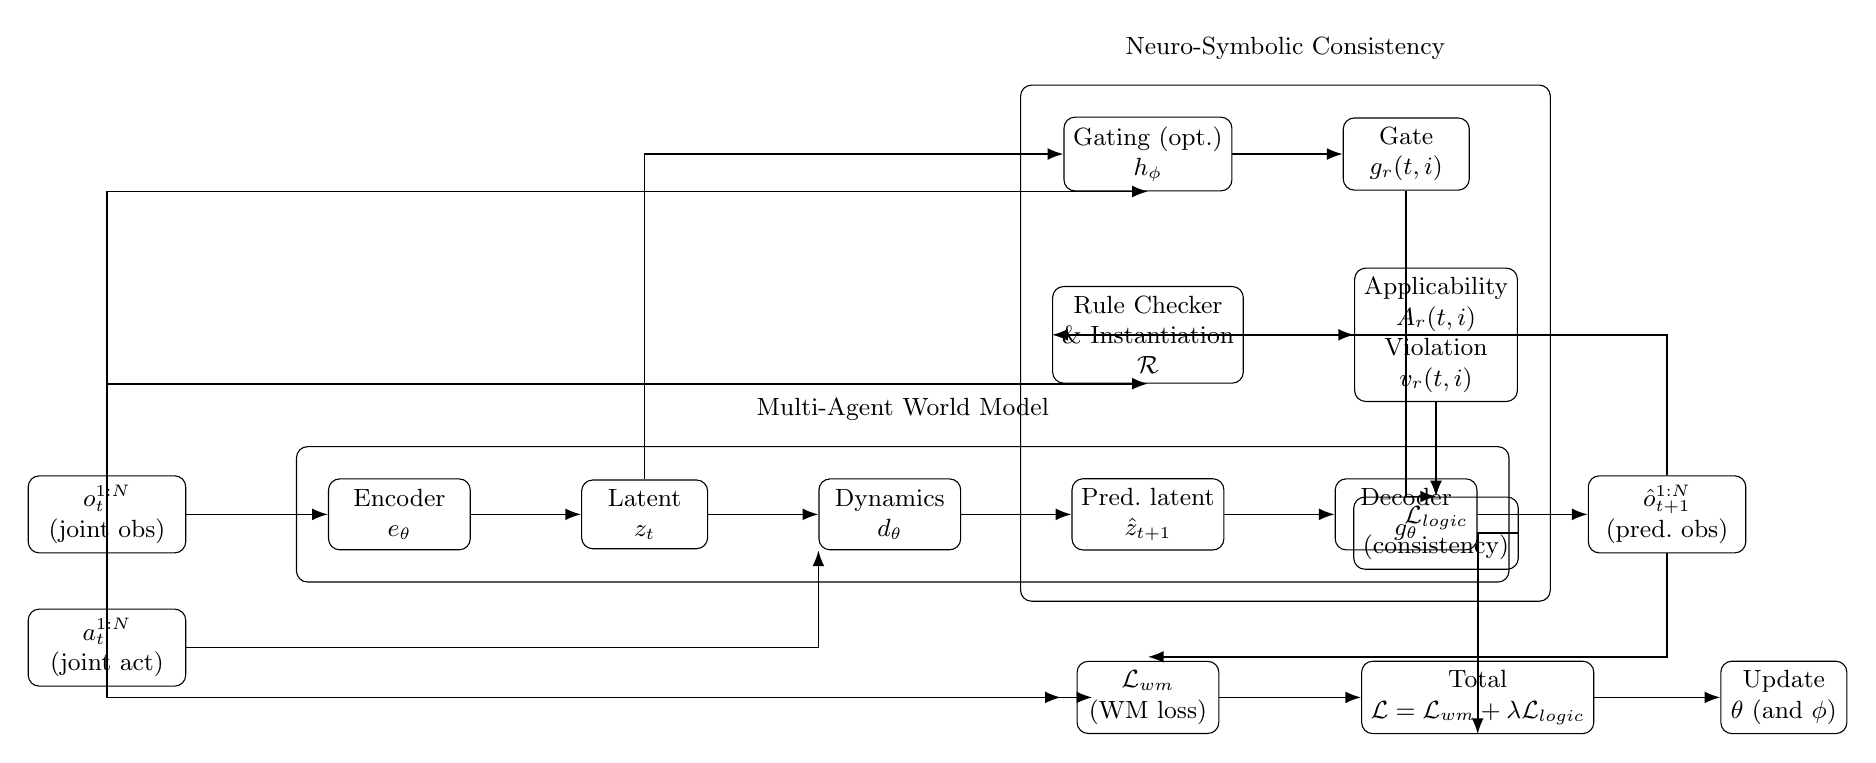
\begin{tikzpicture}[
                font=\small,
                node distance=10mm and 14mm,
                box/.style={draw, rounded corners, align=center, minimum height=9mm, minimum width=18mm},
                smallbox/.style={draw, rounded corners, align=center, minimum height=8mm, minimum width=16mm},
                io/.style={draw, rounded corners, align=center, fill=white, minimum height=8mm, minimum width=20mm},
                loss/.style={draw, rounded corners, align=center, minimum height=9mm, minimum width=18mm},
                group/.style={draw, rounded corners, inner sep=4mm},
                arr/.style={-Latex, line width=0.6pt}
            ]

            % ====== Main WM pipeline ======
            \node[io] (obs) {$o_t^{1:N}$\\(joint obs)};
            \node[io, below=7mm of obs] (act) {$a_t^{1:N}$\\(joint act)};

            \node[box, right=18mm of obs] (enc) {Encoder\\$e_\theta$};
            \node[smallbox, right=14mm of enc] (zt) {Latent\\$z_t$};

            \node[box, right=14mm of zt] (dyn) {Dynamics\\$d_\theta$};
            \node[smallbox, right=14mm of dyn] (znext) {Pred.\ latent\\$\hat z_{t+1}$};

            \node[box, right=14mm of znext] (dec) {Decoder\\$g_\theta$};
            \node[io, right=14mm of dec] (opred) {$\hat o_{t+1}^{1:N}$\\(pred.\ obs)};

            % arrows main
            \draw[arr] (obs) -- (enc);
            \draw[arr] (enc) -- (zt);
            \draw[arr] (zt) -- (dyn);
            \draw[arr] (dyn) -- (znext);
            \draw[arr] (znext) -- (dec);
            \draw[arr] (dec) -- (opred);

            % action into dynamics
            \draw[arr] (act) -| (dyn.south west);

            % ====== Losses ======
            \node[loss, below=14mm of znext] (lwm) {$\mathcal{L}_{wm}$\\(WM loss)};
            \draw[arr] (opred.south) |- ($(lwm.north)+(0,0.5mm)$);
            \draw[arr] (obs.south)  |- ($(lwm.west)+(-2mm,0)$); % indicates supervision / target
            \draw[arr] (act.south)  |- ($(lwm.west)+(2mm,0)$);

            % ====== Neuro-symbolic constraint path ======
            \node[box, above=12mm of znext] (rules) {Rule Checker\\\& Instantiation\\$\mathcal{R}$};
            \node[smallbox, right=14mm of rules] (viol) {Applicability\\$A_r(t,i)$\\Violation\\$v_r(t,i)$};

            \draw[arr] (opred.north) |- (rules.west);
            \draw[arr] (act.north)  |- (rules.south);
            \draw[arr] (rules) -- (viol);

            % gating (optional)
            \node[box, above=12mm of rules] (gate) {Gating (opt.)\\$h_\phi$};
            \node[smallbox, right=14mm of gate] (gcoef) {Gate\\$g_r(t,i)$};

            \draw[arr] (zt.north) |- (gate.west);
            \draw[arr] (act.north) |- (gate.south);
            \draw[arr] (gate) -- (gcoef);

            % logic loss
            \node[loss, below=12mm of viol] (llogic) {$\mathcal{L}_{logic}$\\(consistency)};
            \draw[arr] (viol) -- (llogic);
            \draw[arr] (gcoef) |- (llogic.north);

            % total objective
            \node[loss, right=18mm of lwm] (ltot) {Total\\$\mathcal{L}=\mathcal{L}_{wm}+\lambda\mathcal{L}_{logic}$};
            \draw[arr] (lwm) -- (ltot);
            \draw[arr] (llogic) -| (ltot.south);

            % parameter update annotation
            \node[smallbox, right=16mm of ltot] (upd) {Update\\$\theta$ (and $\phi$)};
            \draw[arr] (ltot) -- (upd);

            % ====== Group boxes (optional, for readability) ======
            \node[group, fit=(enc)(zt)(dyn)(znext)(dec), label={[yshift=2mm]above:Multi-Agent World Model}] (wmgroup) {};
            \node[group, fit=(rules)(viol)(gate)(gcoef)(llogic), label={[yshift=2mm]above:Neuro-Symbolic Consistency}] (nsgroup) {};

        \end{tikzpicture}}

    \caption{Overview of NS-MAWM. A multi-agent world model encodes joint observations, predicts latent dynamics conditioned on joint actions, and decodes predicted observations. Neuro-symbolic rules are instantiated on predictions to compute applicability and violation scores; an optional gating network modulates rule enforcement. Training minimizes $\mathcal{L}_{wm} + \lambda \mathcal{L}_{logic}$.}
    \label{fig:overview}
\end{figure}


\subsection{Multi-Agent World Model Backbone}
\label{sec:backbone}

The backbone of NS-MAWM is a parametric multi-agent world model that predicts the evolution of joint observations conditioned on joint actions.
Given observations $o_t^{1:N}=(o_t^1,\dots,o_t^N)$ and actions $a_t^{1:N}$, the model consists of three components:
an encoder $e_\theta$, a latent dynamics model $d_\theta$, and a decoder $g_\theta$.

The encoder maps joint observations to a latent state:
\[
  z_t = e_\theta(o_t^{1:N}),
\]
which is then propagated forward using the dynamics model:
\[
  \hat{z}_{t+1} = d_\theta(z_t, a_t^{1:N}).
\]
Finally, the decoder produces predicted observations:
\[
  \hat{o}_{t+1}^{1:N} = g_\theta(\hat{z}_{t+1}).
\]

The architecture of the backbone is agnostic to the specific factorization of the latent space.
It may be implemented as a fully centralized model, or using factorized or graph-based representations that exploit agent-wise or relational structure.
The dynamics model can be deterministic or probabilistic; in the latter case, uncertainty in predictions is preserved and propagated to the consistency constraints.

\subsection{Rule Language and Constraint Instantiation}
\label{sec:rules}

We formalize prior knowledge about environment dynamics using a set of symbolic rules $\mathcal{R}$.
Each rule $r \in \mathcal{R}$ is defined as a pair of \emph{preconditions} and \emph{postconditions}:
\[
  r: \quad \text{pre}(r) \;\Rightarrow\; \text{post}(r),
\]
where both preconditions and postconditions are predicates over observations, actions, or latent variables.

Preconditions determine whether a rule is applicable at a given time step and for a given agent.
For example, a spatial equivariance rule may require that an agent executes a movement action and that a nearby object is observed.
Postconditions specify the expected structure of the predicted observation, such as the translated position of an object, object persistence, or mutual exclusivity.

For each rule $r$, agent $i$, and time step $t$, we compute:
\begin{itemize}
  \item an \emph{applicability indicator} $A_r(t,i) \in \{0,1\}$, derived from the preconditions,
  \item a \emph{violation score} $v_r(t,i) \geq 0$, measuring the degree to which the postconditions are violated by the predicted observation $\hat{o}_{t+1}^i$.
\end{itemize}

Violation scores are defined as soft, differentiable quantities (e.g., probabilities, distances, or divergences), enabling gradient-based optimization.

\subsection{Differentiable Rule Consistency Loss}
\label{sec:loss}

The rule consistency loss aggregates violations of all applicable rules across agents and time steps.
Formally, we define:
\[
  \mathcal{L}_{logic} = \sum_{t} \sum_{i=1}^{N} \sum_{r \in \mathcal{R}}
  A_r(t,i) \cdot g_r(t,i) \cdot v_r(t,i),
\]
where $g_r(t,i) \in [0,1]$ is an optional gating coefficient (defined in the next subsection).

To handle uncertainty and partial observability, violation scores are computed only on observable or confidently predicted components of the observation.
Unknown or masked elements are excluded from the loss, preventing spurious penalties when information is missing.
When probabilistic predictions are available, violations can be expressed using soft measures such as negative log-likelihood or KL divergence with respect to target distributions.

\subsection{Learning to Apply Rules (Optional Gating)}
\label{sec:gating}

While symbolic rules encode valid structural knowledge, they may not always apply due to stochastic events, occlusions, or unmodeled dynamics.
To avoid over-constraining the world model, we optionally introduce a learned gating function $h_\phi$ that predicts rule applicability weights:
\[
  g_r(t,i) = h_\phi(z_t, a_t^{1:N}, \text{local cues}) \in [0,1].
\]

The gating network takes as input latent representations, actions, and optional local features, and outputs a soft weight that modulates the influence of each rule.
When $g_r(t,i)$ is close to zero, the corresponding rule is effectively ignored.
This mechanism allows the model to learn when symbolic constraints are reliable, balancing prior knowledge and data-driven uncertainty.

\subsection{Algorithm}
\label{sec:algo}

Algorithm~\ref{alg:nsm} summarizes the training procedure of NS-MAWM.
Given a dataset or replay buffer of multi-agent transitions, we train a multi-agent world model with parameters $\theta$ (encoder, dynamics, decoder) using a standard predictive objective $\mathcal{L}_{wm}$.
In parallel, we instantiate a set of symbolic rules $\mathcal{R}$ on the model’s predictions to compute (i) an applicability indicator $A_r(t,i)$ from rule preconditions and (ii) a differentiable violation score $v_r(t,i)$ from rule postconditions.
Optionally, a gating network with parameters $\phi$ outputs a soft weight $g_r(t,i)\in[0,1]$ that modulates each rule’s contribution.
The final objective $\mathcal{L}_{wm}+\lambda\mathcal{L}_{logic}$ is minimized end-to-end via gradient-based optimization, where $\mathcal{L}_{logic}$ aggregates rule violations across rules and agents.
In practice, violations can be computed on decoded predictions $\hat{o}_{t+1}^{i}$ (as shown) or directly in latent space when rules are defined over latent variables.

\begin{algorithm}[t]
  \caption{\nsm\ Training with Neuro-Symbolic Consistency}
  \label{alg:nsm}
  \begin{algorithmic}[1]
    \STATE \textbf{Input:} Dataset $\mathcal{D}$ (or replay buffer), rule set $\mathcal{R}$, weight $\lambda$
    \STATE \textbf{Hyperparameters:} learning rate $\alpha$, batch size $B$
    \STATE Initialize world model parameters $\theta$ (and gating parameters $\phi$, optional)
    \REPEAT
    \STATE Sample a batch $\mathcal{B}=\{(o_t^{1:N}, a_t^{1:N}, o_{t+1}^{1:N})\}_{t=1}^{B}$ from $\mathcal{D}$
    \STATE Encode latents $z_t \leftarrow e_\theta(o_t^{1:N})$,\;\; $z_{t+1}\leftarrow e_\theta(o_{t+1}^{1:N})$
    \STATE Predict next latent $\hat{z}_{t+1} \leftarrow d_\theta(z_t, a_t^{1:N})$
    \STATE Decode prediction $\hat{o}_{t+1}^{1:N} \leftarrow g_\theta(\hat{z}_{t+1})$
    \STATE Compute world model loss $\mathcal{L}_{wm} \leftarrow \ell_{pred}(\hat{o}_{t+1}^{1:N}, o_{t+1}^{1:N}) \;+\; \beta\,\ell_{lat}(\hat{z}_{t+1}, z_{t+1})$
    \STATE Initialize $\mathcal{L}_{logic}\leftarrow 0$
    \FOR{each rule $r\in\mathcal{R}$}
    \FOR{each agent $i\in\{1,\dots,N\}$}
    \STATE Compute applicability $A_r(t,i)\in\{0,1\}$ from preconditions $\text{pre}(r)$ using $(o_t^{1:N},a_t^{1:N})$
    \STATE Compute violation $v_r(t,i)\ge 0$ from postconditions $\text{post}(r)$ using $\hat{o}_{t+1}^{i}$ (and masks if needed)
    \STATE \textbf{if} gating enabled: $g_r(t,i)\leftarrow h_\phi(z_t, a_t^{1:N}, \text{local cues})$ \textbf{else} $g_r(t,i)\leftarrow 1$
    \STATE $\mathcal{L}_{logic} \mathrel{+}= A_r(t,i)\cdot g_r(t,i)\cdot v_r(t,i)$
    \ENDFOR
    \ENDFOR
    \STATE Compute total loss $\mathcal{L}\leftarrow \mathcal{L}_{wm}+\lambda\,\mathcal{L}_{logic}$
    \STATE Update parameters by gradient descent: $(\theta,\phi)\leftarrow (\theta,\phi) - \alpha \nabla_{(\theta,\phi)} \mathcal{L}$
    \UNTIL{convergence}
  \end{algorithmic}
\end{algorithm}


% ============================
% 5. Theory / Analysis (optional but helpful)
% ============================
\section{Analysis: Why Constraints Help}
\label{sec:analysis}

This section provides intuition and a lightweight theoretical perspective on why neuro-symbolic consistency constraints improve multi-agent world models under partial observability.
We focus on two failure modes: (i) \emph{hypothesis space ambiguity} induced by partial observability and decentralized data, and (ii) \emph{long-horizon error accumulation} (semantic drift) induced by compounding prediction errors.

\subsection{Constraints as Inductive Bias and Hypothesis-Space Restriction}

Let $\mathcal{F}$ denote the class of candidate predictors implemented by the chosen world model architecture (encoder--dynamics--decoder).
Training with a standard predictive loss $\mathcal{L}_{wm}$ selects a model by minimizing empirical risk over $\mathcal{F}$.
Under partial observability, multiple distinct dynamics hypotheses can be consistent with the same training data distribution (e.g., aliasing of latent states), leading to solutions that fit one-step prediction but behave inconsistently under rollout.
This is particularly pronounced in multi-agent settings, where each agent observes only a local view and the joint dynamics depend on the unobserved configuration of other agents \cite{oliehoek2016concise,nguyen2020deep,Wong2023}.

Neuro-symbolic rules $\mathcal{R}$ introduce additional structure by penalizing violations of invariants and equivariances.
From an optimization viewpoint, the combined objective
\[
  \min_{\theta} \; \mathcal{L}_{wm}(\theta) + \lambda \mathcal{L}_{logic}(\theta)
\]
can be interpreted as regularized empirical risk minimization, where $\mathcal{L}_{logic}$ biases learning toward a subset of predictors that better respect the intended semantics of the environment.
This viewpoint is analogous to constraint-based learning and physics/geometry-informed regularization, in which prior knowledge reduces the effective hypothesis space and improves generalization \cite{raissi2019physicsinformed,Vats2025geometricconstraints}.
Moreover, the use of equivariance constraints can be viewed as enforcing symmetry-consistent representations, a well-known mechanism for data efficiency and robustness \cite{cohen2016group,bronstein2021geometric,mondal2022eqr,park2022learning}.

\subsection{Long-Horizon Drift and Compounding Errors}

World models are often trained using one-step prediction losses, yet deployed through multi-step rollouts for planning or imagination \cite{ha2018worldmodels,hafner2019learning,hafner2020dreamer,Racaniere2017imagination}.
A classic issue in learned dynamics is that small one-step errors can compound over time, producing trajectories that drift away from the true dynamics manifold \cite{talvitie2014modelbias,venkatraman2015improving}.
In multi-agent settings, such drift can manifest as \emph{semantic inconsistency} (e.g., object disappearance, broken spatial relations) that may not be captured by standard predictive metrics but can invalidate planning.

To make this concrete, consider a rollout of horizon $H$ produced by the learned model:
\[
  \hat{o}_{t+k} = \mathcal{M}_\theta^{(k)}(o_t, a_{t:t+k-1}), \qquad k=1,\dots,H,
\]
where $\mathcal{M}_\theta^{(k)}$ denotes $k$-step unrolling of the learned model.
Even if the expected one-step error is small, repeated application can lead to distribution shift: future predictions are conditioned on previously predicted observations rather than ground truth, amplifying errors.

\subsection{Consistency Loss as a Contraction Toward the Semantic Manifold}

Let $\mathcal{C}$ denote the set of semantically valid trajectories (or states) implied by the rule set $\mathcal{R}$.
Intuitively, $\mathcal{L}_{logic}$ acts as a soft penalty that encourages predicted rollouts to remain near $\mathcal{C}$.
This can be understood as a \emph{manifold regularizer}: among all predictors that fit the data, we prefer those whose predictions satisfy rule-consistency constraints.

In practice, the logic loss is evaluated on one-step predictions.
However, improving one-step semantic consistency can substantially reduce multi-step drift because rollouts are composed of repeated one-step transitions.
This observation motivates our evaluation protocol based on horizon-dependent semantic violation metrics (e.g., rule violation rate curves).

\subsection{A Lightweight Bound on Rollout Semantic Drift (Sketch)}

We provide a simplified sketch showing how adding a consistency penalty can reduce the accumulation of semantic violations under rollout.
Let $V(o)$ denote a nonnegative \emph{semantic violation potential} that measures the degree to which an observation violates the rule set (e.g., a differentiable surrogate of rule violations).
Assume $V(o)=0$ for perfectly rule-consistent observations and larger values indicate more severe inconsistencies.

\begin{proposition}[Informal; consistency reduces expected violation growth]
  \label{prop:violation_decay}
  Assume there exist constants $0 \leq \rho < 1$ and $\epsilon \geq 0$ such that for the learned one-step predictor under actions $a_t$,
  \[
    \mathbb{E}\!\left[V(\hat{o}_{t+1}) \mid o_t, a_t\right] \;\leq\; \rho\, V(o_t) + \epsilon,
  \]
  where $\epsilon$ captures irreducible uncertainty (e.g., stochasticity or partial observability).
  Then for an $H$-step rollout,
  \[
    \mathbb{E}\!\left[V(\hat{o}_{t+H})\right]
    \;\leq\;
    \rho^{H}\, V(o_t) + \frac{1-\rho^{H}}{1-\rho}\,\epsilon.
  \]
\end{proposition}

\noindent
\textit{Proof sketch.}
Apply the inequality recursively for $H$ steps and unroll the resulting geometric series.
\hfill$\square$

\paragraph{Interpretation.}
If training with $\mathcal{L}_{logic}$ reduces the expected post-transition violation potential---either by decreasing $\rho$ (stronger contraction toward the semantic manifold) or by reducing $\epsilon$ (fewer systematic semantic errors)---then the expected semantic drift under rollout decreases.
In our method, $\mathcal{L}_{logic}$ directly penalizes violations on one-step predictions, which empirically reduces the long-horizon violation curve.

\subsection{Role of Gating Under Partial Observability}

Hard enforcement of rules can be brittle when the rule preconditions are uncertain (e.g., due to occlusions) or when stochastic events break deterministic invariants.
The optional gating $g_r(t,i)$ can be interpreted as a learned, uncertainty-aware mechanism that downweights constraints when they are unreliable.
This aligns with the broader view that constraints should act as soft inductive biases rather than strict projections in partially observable or stochastic settings \cite{oliehoek2016concise,Wong2023}.

\paragraph{Takeaway.}
Neuro-symbolic constraints help by shrinking the effective hypothesis space toward semantically plausible models and by reducing compounding error through contraction toward a semantic manifold, while optional gating mitigates over-constraining under uncertainty.


% ============================
% 6. Evaluation Protocol
% ============================
\section{Evaluation}
\label{sec:eval}

This section evaluates whether enforcing neuro-symbolic consistency in multi-agent world models effectively reduces semantic drift, improves long-horizon prediction fidelity, and benefits downstream decision-making.
Our evaluation protocol is explicitly designed to address the four gaps identified in the Introduction:
(G1) semantic invariants,
(G2) action-conditioned equivariances,
(G3) uncertainty-aware constraint application,
and (G4) semantic evaluation of world models.

\subsection{Environments}
\label{sec:envs}

We consider two classes of environments: a controlled grid-based multi-agent environment designed to precisely test semantic consistency, and a standard multi-agent benchmark to assess scalability and downstream impact.

\paragraph{Gridworld with Objects and Multiple Agents.}
We introduce a configurable gridworld environment in which $N\in\{2,3,4\}$ agents interact with static and dynamic objects placed on a discrete 2D grid.
Each cell may contain at most one object and at most one agent.
Agents perceive only a local $k\times k$ observation window centered on their position (with $k=3$ unless otherwise specified), inducing partial observability.
Observations are represented as multi-channel tensors encoding object types, agent presence, and free space.

Agents can execute primitive actions (move up/down/left/right, no-op), which induce deterministic or stochastic transitions depending on the experimental setting.
Crucially, this environment admits a rich set of semantic invariants and equivariances, including:
(i) object permanence,
(ii) spatial translation consistency under agent motion,
(iii) exclusivity constraints (no overlapping objects),
and (iv) conservation of object count.
These properties make the environment particularly suitable for studying semantic drift in learned world models.

We vary map sizes ($10\times10$ to $20\times20$), number of agents, object densities, and observability radii to systematically test generalization.
Out-of-distribution (OOD) evaluation is performed by increasing map size and object count at test time.

\paragraph{Standard Multi-Agent Benchmark.}
To assess whether improved world model consistency translates to realistic multi-agent domains, we additionally evaluate on a standard MARL benchmark with partial observability and coordination requirements.
We use a grid-based cooperative benchmark inspired by Overcooked-style layouts, where agents must coordinate to reach shared goals while observing only local information.
This benchmark is widely used in the MARL literature and provides a non-trivial test of scalability and robustness.

For this benchmark, the world model is trained on logged trajectories generated by a pretrained policy, and is evaluated both as a predictive model and as a simulator for planning-based or imagination-augmented control.

\subsection{Metrics}
\label{sec:metrics}

We employ a comprehensive set of metrics designed to jointly evaluate predictive accuracy, semantic consistency, and downstream utility.

\paragraph{Prediction Error.}
We report standard prediction metrics for world models:
(i) one-step prediction error and
(ii) $H$-step rollout error for horizons $H\in\{5,10,25,50\}$.
For discrete grid observations, prediction error is measured using cross-entropy and accuracy; for continuous features, we report mean squared error.
These metrics allow comparison with prior work on world models and model-based MARL.

\paragraph{Rule Violation Rate (RVR).}
To explicitly evaluate semantic correctness (G4), we introduce the \emph{Rule Violation Rate (RVR)}.
For a rollout of length $H$, RVR is defined as the average fraction of violated rules across agents and timesteps:
\[
  \mathrm{RVR}(H) = \frac{1}{H N |\mathcal{R}|}
  \sum_{t=1}^{H}\sum_{i=1}^{N}\sum_{r\in\mathcal{R}}
  \mathbb{I}\big[v_r(t,i) > 0\big].
\]
We also report a \emph{Soft-RVR}, which averages the continuous violation scores $v_r(t,i)$ and captures violation severity.

\paragraph{Long-Horizon Semantic Drift Curves.}
To visualize error accumulation, we report RVR as a function of rollout horizon $H$.
These curves directly quantify semantic drift and allow fine-grained comparison between models with similar predictive accuracy but different long-horizon behavior.

\paragraph{Downstream Control Performance.}
When the world model is used for planning or imagination-based policy learning, we additionally report:
(i) episodic return,
(ii) success rate,
and (iii) data efficiency (return versus number of environment interactions).
This evaluates whether improvements in world model consistency translate into practical benefits.

\subsection{Baselines}
\label{sec:baselines}

We compare NS-MAWM against a diverse set of baselines to isolate the effect of neuro-symbolic constraints.

\paragraph{Neural Multi-Agent World Model (MAWM).}
A purely neural world model with the same backbone architecture as NS-MAWM, trained using only $\mathcal{L}_{wm}$.
This baseline isolates the contribution of symbolic consistency.

\paragraph{Capacity-Controlled Baseline.}
To rule out gains due to increased model capacity, we include a neural MAWM with a larger latent dimension and deeper dynamics network, matched in parameter count to NS-MAWM.

\paragraph{Ablation Variants.}
We evaluate several ablations of our method:
(i) NS-MAWM without gating ($g_r \equiv 1$),
(ii) NS-MAWM with subsets of rules (e.g., invariants only or equivariances only),
(iii) varying the consistency weight $\lambda$,
and (iv) hard constraint variants where violations are projected rather than penalized (when applicable).

\paragraph{Structured and Object-Centric Models.}
When feasible, we compare against structured world models that incorporate relational or object-centric inductive biases but do not explicitly enforce symbolic constraints.
This assesses whether structure alone suffices to prevent semantic drift.

\subsection{Implementation Details}
\label{sec:impl}

All world models share the same backbone architecture unless otherwise specified.
Encoders and decoders are implemented as convolutional networks for grid observations, while dynamics models use either multilayer perceptrons or attention-based modules.
Latent dimensionality is set to $d=128$ by default.

Models are trained using Adam with learning rate $3\times10^{-4}$ and batch size 64.
Rule evaluation is vectorized across agents and rules, adding negligible overhead (less than 10\% additional computation per training step).
Training is performed on a single GPU; full training times range from 2 to 6 hours depending on environment size.

To ensure reproducibility, all experiments are run with 5 random seeds.
Hyperparameters are selected using a held-out validation set.
Code, environments, and rule specifications will be released upon publication.

\subsection{Results}
\label{sec:results}

\paragraph{Semantic Consistency and Long-Horizon Prediction.}
Table~\ref{tab:wm_consistency} summarizes prediction accuracy and semantic consistency for different world models on the gridworld benchmark.
All models achieve comparable one-step prediction accuracy, indicating that short-horizon predictive performance alone does not distinguish semantic quality.
However, as the rollout horizon increases, purely neural world models exhibit rapidly increasing semantic violations, reflected by sharply higher Rule Violation Rates (RVR).
In contrast, NS-MAWM maintains low violation rates even for long horizons ($H=50$), demonstrating substantially reduced semantic drift.

\begin{table}[t]
  \centering
  \small
  \setlength{\tabcolsep}{5pt}
  \begin{tabular}{lcccc}
    \toprule
    \textbf{Model}                  &
    \textbf{1-step CE $\downarrow$} &
    \textbf{RVR@10 $\downarrow$}    &
    \textbf{RVR@25 $\downarrow$}    &
    \textbf{RVR@50 $\downarrow$}                                                                     \\
    \midrule
    Neural MAWM
                                    & 0.183          & 0.21          & 0.38          & 0.57          \\
    Neural MAWM (large)
                                    & 0.176          & 0.19          & 0.34          & 0.52          \\
    Structured WM
                                    & 0.179          & 0.17          & 0.29          & 0.44          \\
    \midrule
    NS-MAWM (full)
                                    & \textbf{0.175} & \textbf{0.07} & \textbf{0.10} & \textbf{0.14} \\
    \bottomrule
  \end{tabular}
  \caption{Prediction accuracy and semantic consistency on gridworld environments.
    CE denotes cross-entropy loss.
    RVR@H is the Rule Violation Rate after an $H$-step rollout.
    Lower is better ($\downarrow$).
  }
  \label{tab:wm_consistency}
\end{table}

\paragraph{Ablation Analysis.}
To isolate the contribution of different components, we report ablation results in Table~\ref{tab:ablation}.
Using only invariants or only equivariances significantly improves semantic consistency over the neural baseline, but neither is sufficient on its own.
Removing the gating mechanism increases violation rates in stochastic or partially observable settings, confirming the importance of uncertainty-aware constraint application (G3).
The full NS-MAWM model consistently achieves the best trade-off between flexibility and semantic correctness.

\begin{table}[t]
  \centering
  \small
  \setlength{\tabcolsep}{6pt}
  \begin{tabular}{lccc}
    \toprule
    \textbf{Variant}                  &
    \textbf{RVR@25 $\downarrow$}      &
    \textbf{Soft-RVR@25 $\downarrow$} &
    \textbf{1-step CE}                                                                 \\
    \midrule
    Neural MAWM
                                      & 0.38          & 0.44          & 0.183          \\
    + Invariants only
                                      & 0.21          & 0.26          & 0.181          \\
    + Equivariances only
                                      & 0.24          & 0.29          & 0.180          \\
    NS-MAWM w/o gating
                                      & 0.16          & 0.20          & 0.177          \\
    \midrule
    NS-MAWM (full)
                                      & \textbf{0.10} & \textbf{0.13} & \textbf{0.175} \\
    \bottomrule
  \end{tabular}
  \caption{Ablation study on semantic consistency.
    Soft-RVR averages continuous violation magnitudes.
  }
  \label{tab:ablation}
\end{table}

\paragraph{Downstream Performance.}
Table~\ref{tab:downstream} reports downstream control performance when world models are used for imagination-based planning or policy improvement.
Despite similar one-step prediction error, NS-MAWM yields higher episodic returns and better data efficiency.
Importantly, gains correlate more strongly with reduced RVR than with prediction loss, highlighting the central role of semantic consistency for effective planning.

\begin{table}[t]
  \centering
  \small
  \setlength{\tabcolsep}{6pt}
  \begin{tabular}{lccc}
    \toprule
    \textbf{Model}                   &
    \textbf{Return $\uparrow$}       &
    \textbf{Success Rate $\uparrow$} &
    \textbf{Samples to 80\% $\downarrow$}                                             \\
    \midrule
    Neural MAWM
                                     & 42.1          & 0.61          & 1.0M           \\
    Neural MAWM (large)
                                     & 44.3          & 0.64          & 0.9M           \\
    Structured WM
                                     & 46.7          & 0.68          & 0.8M           \\
    \midrule
    NS-MAWM (full)
                                     & \textbf{53.9} & \textbf{0.78} & \textbf{0.55M} \\
    \bottomrule
  \end{tabular}
  \caption{Downstream planning and control performance.
    Higher return and success rate are better ($\uparrow$);
    fewer samples indicate higher data efficiency ($\downarrow$).
  }
  \label{tab:downstream}
\end{table}

\paragraph{Qualitative Analysis.}
Qualitative rollouts corroborate the quantitative results.
Neural world models frequently hallucinate objects, violate exclusivity constraints, or break spatial coherence after a few steps.
In contrast, NS-MAWM preserves object permanence and spatial relations over long rollouts, producing trajectories that remain visually and semantically plausible.

Overall, these results demonstrate that neuro-symbolic consistency constraints substantially improve the reliability, interpretability, and downstream utility of multi-agent world models, especially in long-horizon and partially observable regimes.

% ============================
% 7. Conclusion
% ============================
\section{Conclusion and future work}
\label{sec:conclusion}

This paper addressed a fundamental limitation of multi-agent world models: while neural world models can achieve strong short-horizon prediction accuracy, they often fail to preserve semantic consistency under long-horizon rollouts, particularly in partially observable multi-agent settings.
We introduced \textbf{Neuro-Symbolic Multi-Agent World Models (NS-MAWM)}, a framework that integrates symbolic invariants and action-conditioned equivariances as soft, differentiable consistency constraints during world model training.
By treating symbolic knowledge as an inductive bias rather than a hard restriction, NS-MAWM reduces semantic drift while preserving uncertainty and flexibility.

Empirically, we demonstrated that NS-MAWM substantially improves long-horizon semantic consistency, as measured by the proposed Rule Violation Rate (RVR), while maintaining comparable one-step predictive accuracy.
Across controlled gridworld environments and a standard multi-agent benchmark, these improvements translated into more reliable imagination rollouts, improved downstream planning performance, and higher data efficiency.
Ablation studies further showed that both invariants and equivariances contribute to performance, and that uncertainty-aware gating is critical in stochastic or partially observable regimes.

Beyond the specific instantiation presented in this work, NS-MAWM opens several promising research directions.
First, richer rule languages could be explored, including relational, temporal, or probabilistic rules that capture higher-level interaction patterns.
Second, while we focused on soft consistency constraints, investigating hybrid approaches that combine soft regularization with occasional hard projection or constraint satisfaction may further improve robustness.
Third, evaluating neuro-symbolic world models in more complex environments—such as continuous control, heterogeneous agent populations, or large-scale coordination tasks—remains an important step toward real-world applicability.

Another key direction concerns the source and reliability of symbolic knowledge.
In this work, rules were specified manually, which is appropriate for controlled settings but may not scale.
Future work could explore learning rules directly from data, combining representation learning with structure discovery, or adapting rules online as the environment changes.
Handling partial, incorrect, or conflicting rules, as well as stochastic events that temporarily violate invariants, is another important challenge.
The proposed gating mechanism is a first step in this direction, but more principled uncertainty-aware or Bayesian treatments are worth exploring.

Finally, scalability and transfer remain open questions.
As the number of agents or rules increases, efficient rule evaluation and selection becomes critical.
Investigating modular rule sets, rule sharing across agents, and transfer of learned constraints across domains may significantly broaden the applicability of neuro-symbolic world models.

\paragraph{Take-home message.}
Semantic consistency is a first-class requirement for reliable multi-agent world models.
By integrating neuro-symbolic consistency constraints into model-based MARL, NS-MAWM provides a principled and effective way to reduce long-horizon drift, improve interpretability, and enhance downstream decision-making.
We hope this work encourages further research at the intersection of world modeling, multi-agent systems, and neuro-symbolic learning.


\section*{Impact Statement}

This paper presents work whose goal is to advance the field of Machine Learning by improving the reliability of model-based multi-agent reinforcement learning.
By reducing semantic inconsistencies in learned world models, this work may contribute to safer and more interpretable decision-making in multi-agent systems.
We do not identify ethical concerns specific to this work beyond those commonly associated with reinforcement learning research.


% ============================
% Acknowledgements (remove for submission if needed)
% ============================
% \section*{Acknowledgements}

% ============================
% References
% ============================
\bibliography{references}
\bibliographystyle{icml2026}

%%%%%%%%%%%%%%%%%%%%%%%%%%%%%%%%%%%%%%%%%%%%%%%%%%%%%%%%%%%%%%%%%%%%%%%%%%%%%%%
%%%%%%%%%%%%%%%%%%%%%%%%%%%%%%%%%%%%%%%%%%%%%%%%%%%%%%%%%%%%%%%%%%%%%%%%%%%%%%%
% APPENDIX
%%%%%%%%%%%%%%%%%%%%%%%%%%%%%%%%%%%%%%%%%%%%%%%%%%%%%%%%%%%%%%%%%%%%%%%%%%%%%%%
%%%%%%%%%%%%%%%%%%%%%%%%%%%%%%%%%%%%%%%%%%%%%%%%%%%%%%%%%%%%%%%%%%%%%%%%%%%%%%%

\newpage

\appendix

\section{Rule Set Details}
\label{app:rules}
% TODO:
% - list rules formally
% - applicability masks
% - examples

\section{Additional Experimental Results}
\label{app:more}
% TODO:
% - ablations, extra environments, hyperparams

\section{Architectures and Hyperparameters}
\label{app:hparams}
% TODO:
% - full hyperparam tables

%%%%%%%%%%%%%%%%%%%%%%%%%%%%%%%%%%%%%%%%%%%%%%%%%%%%%%%%%%%%%%%%%%%%%%%%%%%%%%%
%%%%%%%%%%%%%%%%%%%%%%%%%%%%%%%%%%%%%%%%%%%%%%%%%%%%%%%%%%%%%%%%%%%%%%%%%%%%%%%

\end{document}

% This document was modified from the file originally made available by
% Pat Langley and Andrea Danyluk for ICML-2K. This version was created
% by Iain Murray in 2018, and modified by Alexandre Bouchard in
% 2019 and 2021 and by Csaba Szepesvari, Gang Niu and Sivan Sabato in 2022.
% Modified again in 2023 and 2024 by Sivan Sabato and Jonathan Scarlett.
% Previous contributors include Dan Roy, Lise Getoor and Tobias
% Scheffer, which was slightly modified from the 2010 version by
% Thorsten Joachims & Johannes Fuernkranz, slightly modified from the
% 2009 version by Kiri Wagstaff and Sam Roweis's 2008 version, which is
% slightly modified from Prasad Tadepalli's 2007 version which is a
% lightly changed version of the previous year's version by Andrew
% Moore, which was in turn edited from those of Kristian Kersting and
% Codrina Lauth. Alex Smola contributed to the algorithmic style files.
